\subsection{Periodicity Tasks}\label{synth-benchmark:periodicity}

We introduce a family of synthetic tasks designed to evaluate the temporal reasoning capabilities of TGL methods in learning periodic structures. These tasks systematically assess two fundamental cognitive abilities: \emph{counting} (tracking the position within a cycle) and \emph{memorization} (retaining multiple distinct graph patterns). Our benchmark includes both deterministic variants, where exact graph structures repeat, and stochastic variants, where only the underlying generative distributions follow periodic patterns—creating a comprehensive evaluation framework for temporal pattern recognition.


\begin{figure}[ht]
    \centering
    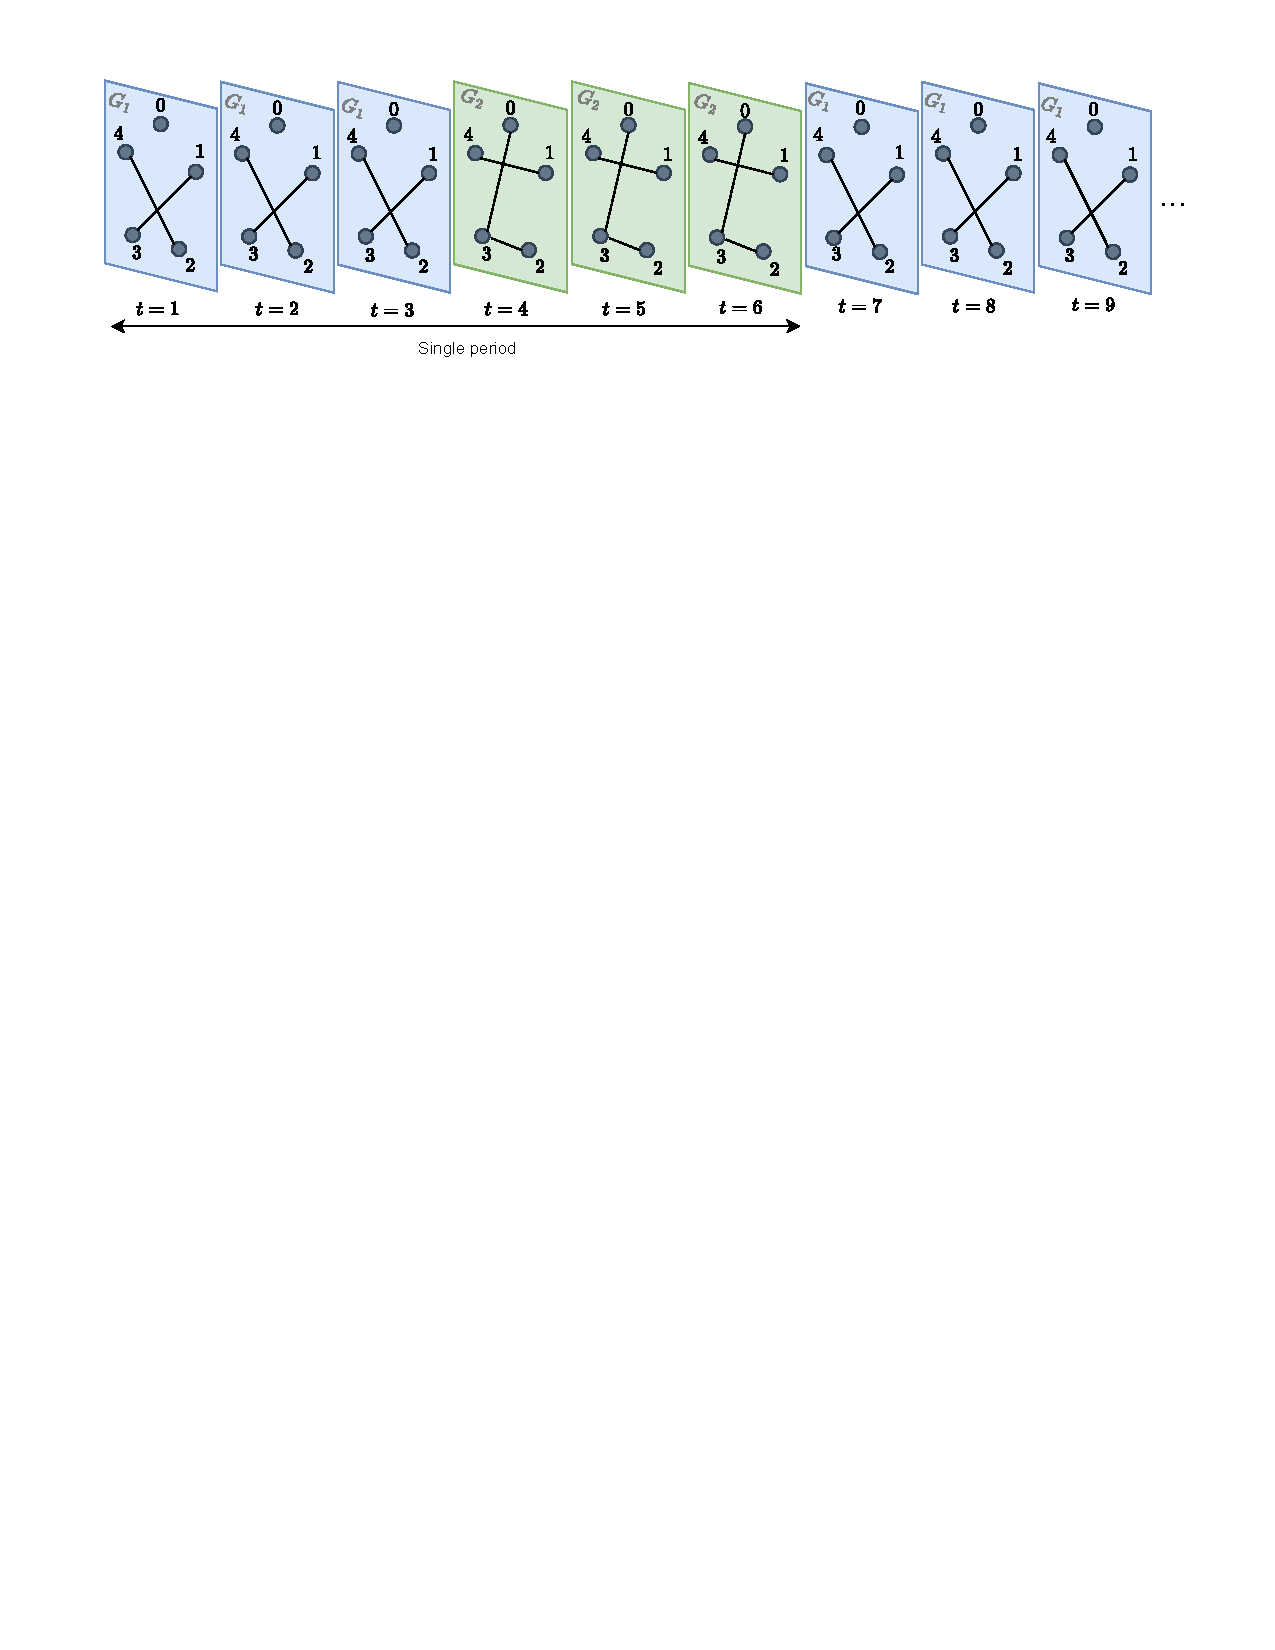
\includegraphics[width=\linewidth, height=8em, keepaspectratio]{figs/periodicity/Fixed_ER/(2, 3)_dataset.pdf}
    \caption{A periodic task in $\Pdet{k=2,n=3}$ containing two unique snapshots, each repeated three times within a single period. }
    \label{fig:periodicity}
\end{figure}


\begin{definition}[Periodicity Tasks]
Let $k, n \in \mathbb{N}$. The task families $\Pdet{k,n}$ and $\Psto{k,n}$ are defined based on a repeating pattern $p$ where each integer $i \in \{1,\dots,k\}$ appears $n$ consecutive times before cycling. At each time step $t$, let $i_t = (\lfloor t/n\rfloor \mod k) + 1$.
In $\Pdet{k,n}$, the dynamic graph $\mathcal{G} = G_1, G_2, \dots$ is a periodic sequence alternating between $k$ fixed static graphs $G_1, \dots, G_k$, i.e., $G_t = G_{i_t}$.
In $\Psto{k,n}$, each $G_t$ is sampled from one of $k$ distributions $D_1, \dots, D_k$ over static graphs (e.g., Erd\H{o}s-Rényi~(ER)~\cite{erdos1960evolution}, Stochastic Block Model~(SBM)~\cite{holland1983stochastic}), with $G_t \sim D_{i_t}$. The resulting sequence is stochastic, but the distribution pattern follows the same periodic structure as in $\Pdet{k,n}$.
\end{definition}

For example, a task in $\Pdet{k=3,n=2}$  will correspond to a dynamic graph $ G_1,G_1,G_2,G_2,$ $G_3,G_3,G_1,G_1,$..., where $G_1,G_2,G_3$ are static graphs. A task  illustration is shown in $\Pdet{k,n}$ is shown in Figure~\ref{fig:periodicity}.



\textbf{Task objectives.}
Tasks in $\Pdet{k,n}$ test the counting and memory capacity of TGL methods. The parameter $k$ controls the length of the pattern and thus the memory demand, while $n$ governs how long each graph is repeated and tests the model's ability to count. For instance, solving a task in $\Pdet{2,n}$ requires counting up to $n$ before switching graphs, while solving a task in $\Pdet{k,1}$ requires memorizing $k$ static graphs. Tasks in $\Psto{k,n}$ introduce stochasticity, requiring models to reason over distributions rather than fixed structures, increasing the complexity while retaining the same periodic structure. 
%Detailed dataset statistics of the dataset we generated for these tasks can be found in \Cref{appendix:periodicity-deterministic-stats}.


\begin{figure}
    \centering
    \begin{subfigure}[b]{0.3\textwidth}
        \centering
        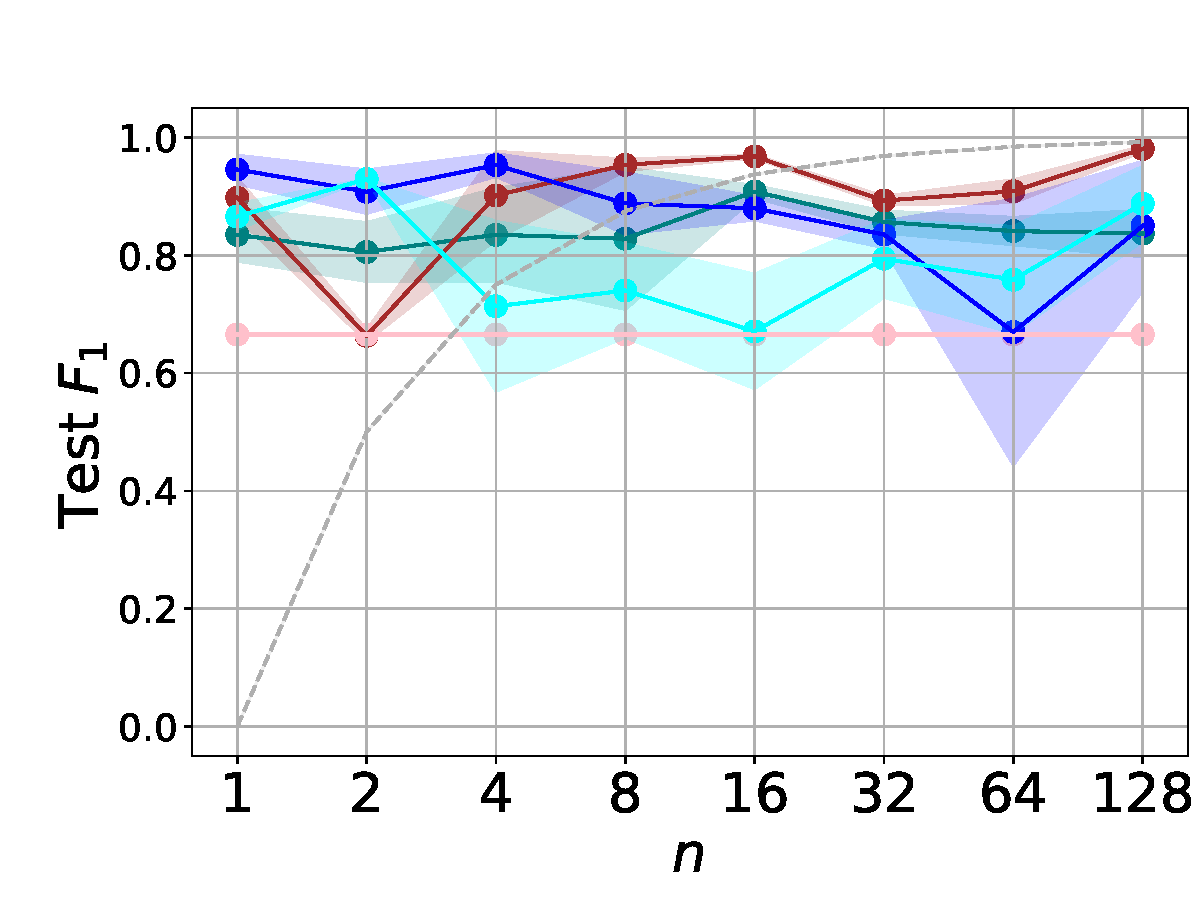
\includegraphics[width=\linewidth,trim={0 2.25cm 0 0},clip]{figs/periodicity/Fixed_ER/(2, n)CTDG_Test $F_1$.pdf}      
        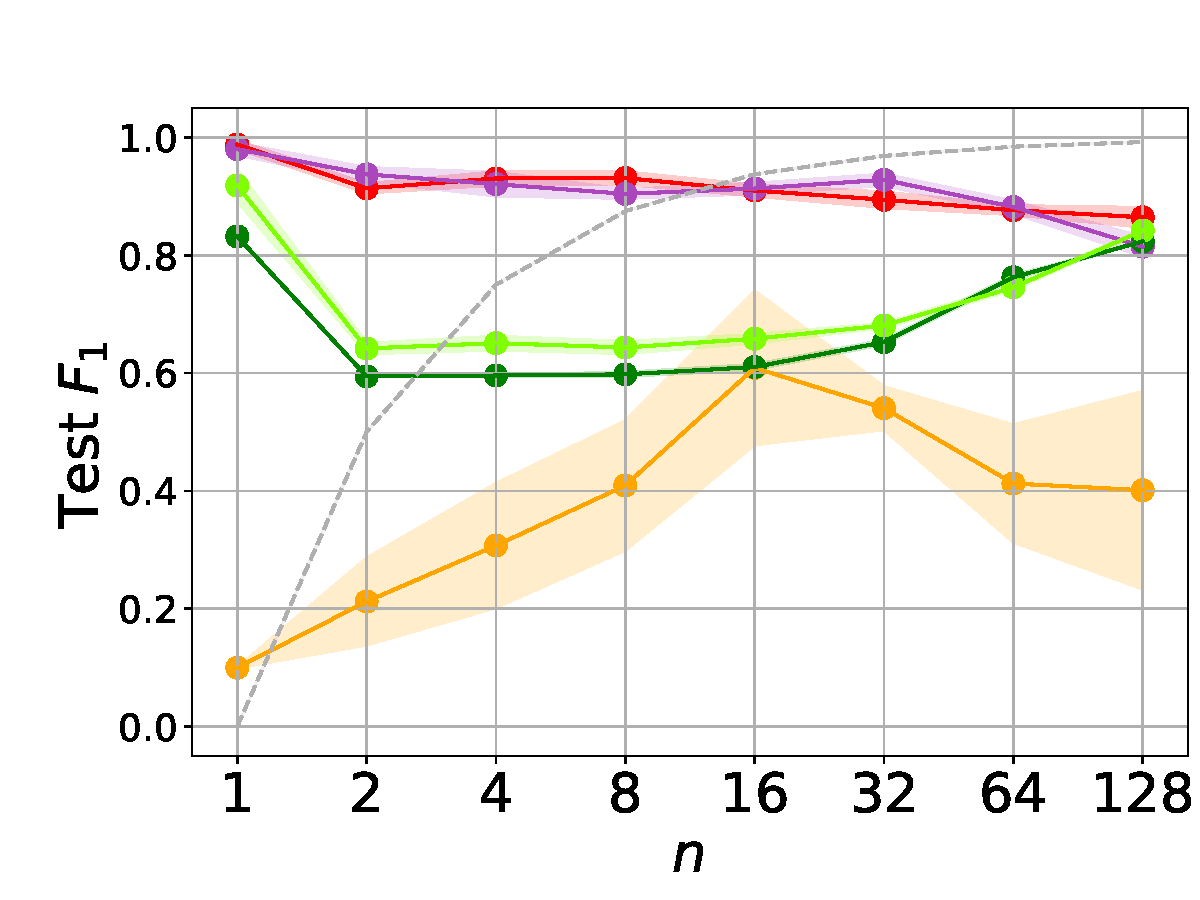
\includegraphics[width=\linewidth,trim={0 0 0 1.2cm },clip]{figs/periodicity/Fixed_ER/(2, n)DTDG_Test $F_1$.pdf}
        \caption{$\Pdet{2,n}$ - All time steps.}
        \label{fig:dtdg_(2,n)_allsteps}
    \end{subfigure}
    \begin{subfigure}[b]{0.3\textwidth}
        \centering
        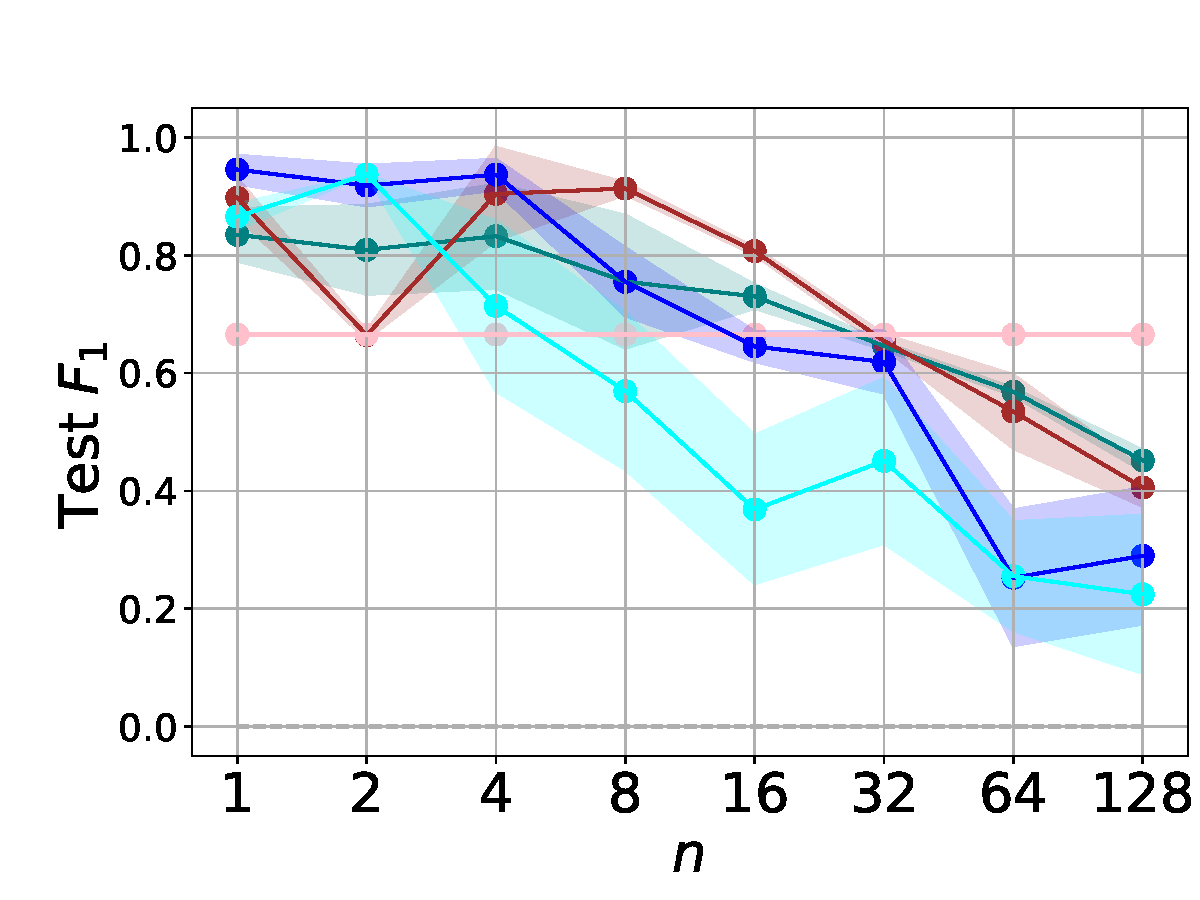
\includegraphics[width=\linewidth,trim={0 2.25cm 0 0},clip]{figs/periodicity/Fixed_ER/change_point/(2, n)CTDG_CP_Test $F_1$.pdf}
        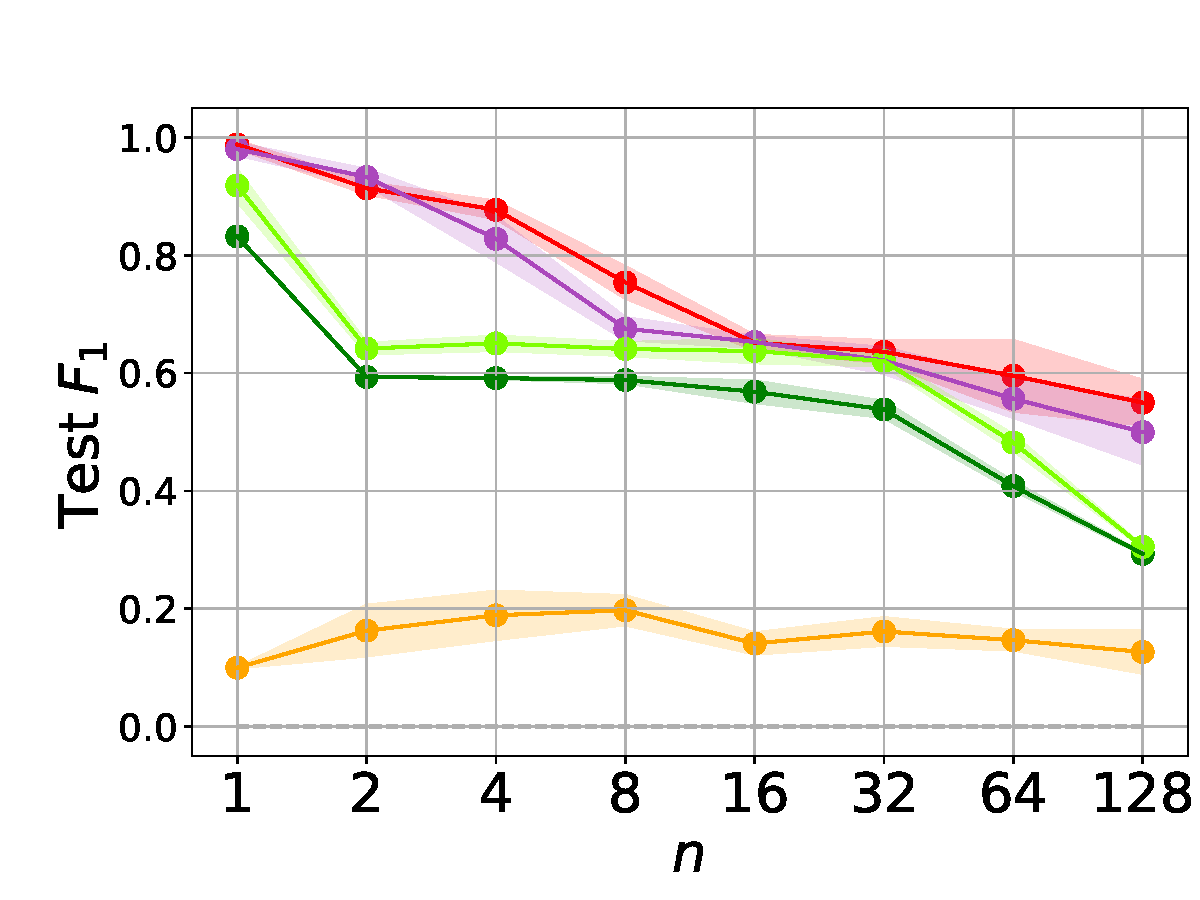
\includegraphics[width=\linewidth,trim={0 0 0 1.2cm },clip]{figs/periodicity/Fixed_ER/change_point/(2, n)DTDG_CP_Test $F_1$.pdf}
        \caption{ $\Pdet{2,n}$ - Change points.}
        \label{fig:dtdg_(2,n)_changepoints}
    \end{subfigure}
    \begin{subfigure}[b]{0.3\textwidth}
        \centering
        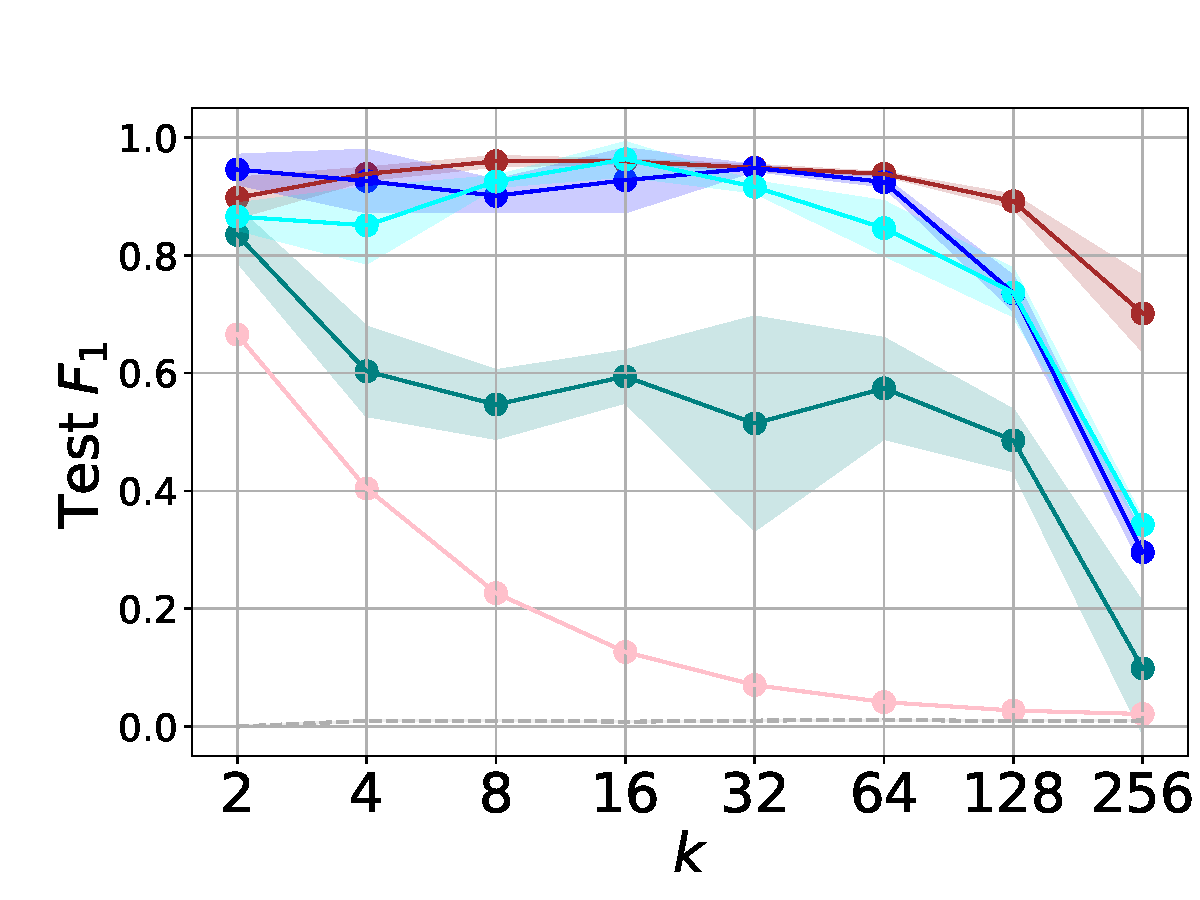
\includegraphics[width=\linewidth,trim={0 2.25cm 0 0},clip]{figs/periodicity/Fixed_ER/(k, 1)CTDG_Test $F_1$.pdf}
        
        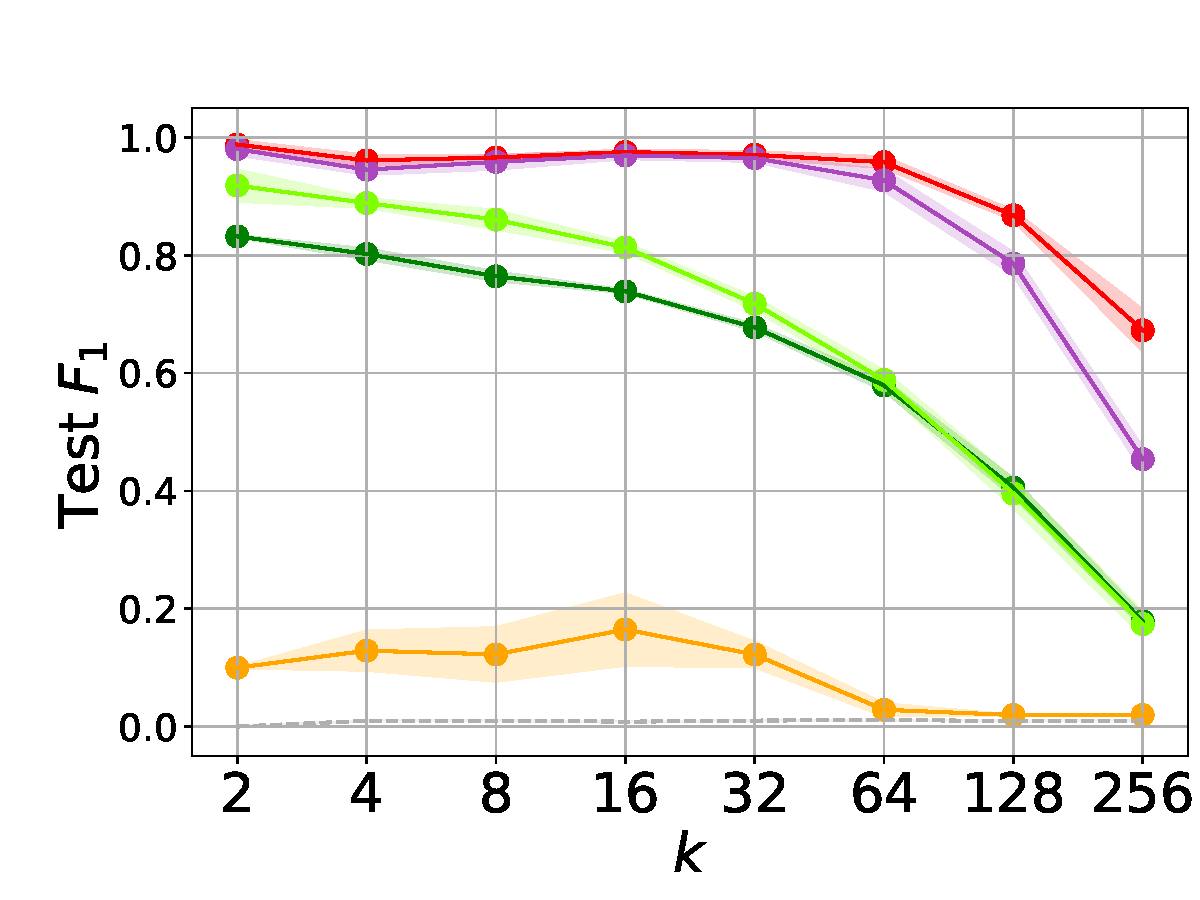
\includegraphics[width=\linewidth,trim={0 0 0 1.2cm },clip]{figs/periodicity/Fixed_ER/(k, 1)DTDG_Test $F_1$.pdf}
        \caption{$\Pdet{k, 1}$ - All time steps.}
        \label{fig:dtdg_(k, 1)}
    \end{subfigure}
    \begin{subfigure}[b]{0.08\textwidth}
        \centering
        \raisebox{14mm}{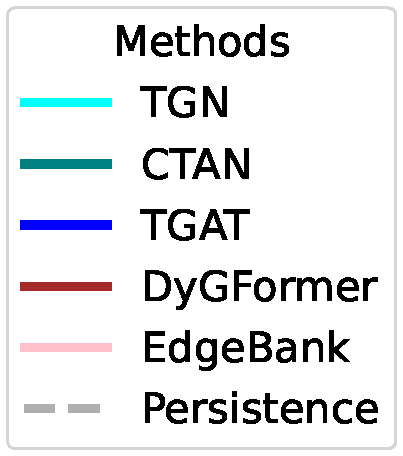
\includegraphics[width=\linewidth]{figs/legends/CTDG w persistence.pdf}}
        
        \raisebox{14mm}{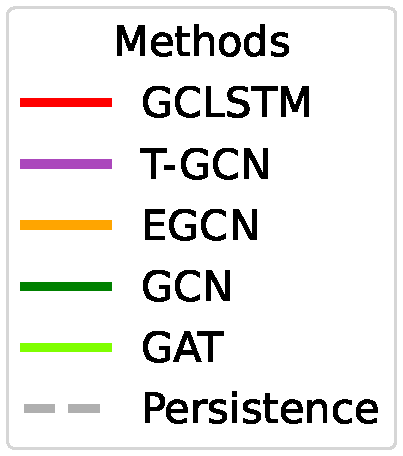
\includegraphics[width=\linewidth]{figs/legends/DTDG w persistence.pdf}}
    \end{subfigure}
    
    \caption{
    Performance of CTDG methods (top row) and DTDG methods (bottom row) on the deterministic periodicity tasks.
    %$\Pdet{2, n}$~(left and center) and $\Pdet{k, 1}$~(right). 
    }
    \label{fig:det_periodic_overall}
\end{figure}




% \at{The following feels out of place?} \ah{I will try rephrasing.}
% \ah{we use $n$ for number of nodes and number of repetions?? notation overload. Do we even need to explain the graph construction for every task?}\gr{No, number of nodes should be $N$}

\looseness-1 \textbf{Can TGNNs count?} To evaluate the counting ability of TGNNs, we construct tasks in $\Pdet{k,n}$ with graphs sampled from the Erdős-Rényi~(ER) model~\citep{erdos1960evolution} (100 nodes, edge probability 0.01). We set $k = 2$ and vary $n$, where increasing $n$ corresponds to greater task difficulty as models must count longer sequences. 
Performance on these $\Pdet{2,n}$ tasks for $n \in \{1,\ldots,128\}$ is presented in \Cref{fig:det_periodic_overall}. We report the $F_1$ score for dynamic link prediction in two critical ways: across all timesteps (left plot) and exclusively at change points (center plot).
Since models that simply repeat the previous timestep can perform well for large $n$, evaluating performance at change points (where the active graph switches, i.e., $t = n+1, 2n+1, \cdots$) is particularly revealing. A high score at change points indicates genuine counting and pattern understanding, whereas high overall performance with poor change point performance suggests the model is merely exploiting temporal continuity rather than reasoning about periodicity.

\looseness-1 The results reveal distinct behavioral patterns across TGNN families. Among CTDG models, TGAT excels for small $n$, while DyGFormer demonstrates more consistent performance as $n$ increases. For DTDG methods, TGCN and GCLSTM achieve the strongest overall results. Notably, EvolveGCN underperforms even static graph learning methods (GCN and GAT), which lack temporal processing mechanisms—highlighting how challenging these seemingly simple periodic patterns can be for current TGNNs. EdgeBank maintains constant performance across all $n$ values by predicting the union of both graphs, making its output invariant to $n$. The persistence baseline improves over all timesteps as $n$ increases by simply copying the previous snapshot, but predictably scores zero at change points.

\looseness-1 A critical insight emerges when comparing performance over all timesteps versus at change points (\Cref{fig:det_periodic_overall}): as $n$ increases, many models increasingly rely on repetition rather than explicit counting. While their overall scores remain high or even improve for larger $n$ (due to successful prediction during extended static phases), their performance at change points often deteriorates or fails to improve proportionally. At $n = 32$, EdgeBank begins to outperform all TGNNs at change points. This divergence suggests that current TGNNs struggle to robustly count long sequences and instead learn simpler heuristics resembling persistence. Further per-timestep analysis supporting this finding is provided in Appendix~\ref{appendix:pertimesteps_counting}.



\looseness-1 \textbf{How much can TGNNs memorize?} To systematically evaluate the memorization capabilities of TGNNs, we fix $n = 1$ and vary $k$, creating a controlled experiment where models must distinguish and recall an increasing number of unique graph structures. This paradigm directly challenges a model's capacity to maintain distinct representations for each graph pattern and correctly anticipate recurring structures in the sequence. \label{seq:memorize}

\looseness-1 Figure~\ref{fig:det_periodic_overall} (right) presents performance on $\Pdet{k, 1}$ across $k \in \{2,\ldots,256\}$. The results reveal clear performance stratification among architectures. GCLSTM and DyGFormer demonstrate superior memorization capacity, maintaining relatively robust performance even at high $k$ values. A second tier comprising TGCN, TGN, and TGAT exhibits strong performance up to $k = 128$ before experiencing precipitous declines at $k = 256$, indicating they reach well-defined memorization thresholds. As anticipated, EdgeBank's performance deteriorates monotonically with increasing $k$, eventually approaching zero at $k = 256$ as it defaults to predicting complete graphs.

\looseness-1 Perhaps most revealing is the performance of certain specialized temporal architectures—notably CTAN and EvolveGCN—which underperform relative to their architectural complexity. CTAN's performance begins deteriorating markedly beyond $k=64$, while EvolveGCN struggles across all $k$ values. Strikingly, both are consistently outperformed by simpler static GNNs (GCN and GAT) that lack explicit temporal processing mechanisms. This counterintuitive finding suggests that poorly designed temporal components can actively interfere with a model's ability to form stable representations of distinct graph states. For tasks primarily requiring state memorization, an ineffective temporal mechanism appears more detrimental than having no temporal processing at all—highlighting the importance of architectural choices that properly balance representational stability with temporal adaptivity.

% % \looseness-1
% To probe the \textit{memorization} capabilities of TGNNs, we can conversely vary $k$ and fix $n = 1$. In this setting, a given model needs to be able to 1) determine which of $G_1 \dots G_k$ is some $G_t$ equal to and 2) \textit{memorize} events in the past to determine what comes next in $k$-length periodic sequence.
% As $k$ increases, the task increases in difficulty as it requires the model to memorize a longer sequence of past events. 

% Figure~\ref{fig:det_periodic_overall}~(right) shows the performance of all methods on the task $\Pdet{k, 1}$ datasets for values of $k$ ranging from 2 to 256. All methods gradually lose memorization ability as $k$ increases. GCLSTM and DyGFormer consistently achieve the highest performance across all values of $k$, demonstrating strong memorization of diverse patterns. TGCN, TGN, and TGAT remain robust up to $k = 128$, but show a significant drop at $k = 256$. Surprisingly, CTAN and  EvolveGCN underperform even compared to static methods like GCN and GAT, which ignore temporal information. As expected, Edgebank performance degrades steadily, reaching zero for $\Pdet{256, 1}$, eventually defaulting to predicting each snapshot as a clique at higher $k$.



% Note that we did not include $k = 1$ as it is a degenerate case with only one graph type in the deterministic case or one distribution in the stochastic case. 
\looseness-1 \textbf{Can TGNNs learn stochastic periodic structures?} Finally, we investigate how models' memorization capabilities extend to probabilistic settings, where periodic structures emerge from underlying stochastic processes rather than deterministic patterns. 
We employ the Stochastic Block Model (SBM) to generate graphs with 100 nodes partitioned into 3 communities. While all SBM distributions maintain consistent intra- and inter-community edge probabilities, they differ in their community structures (detailed in Appendix~\ref{appendix:periodicity_stochastic_design}).
We fix the inter-community edge probability at 0.01 and examine two scenarios for intra-community edge probability $p$: a high-contrast setting ($p=0.9$) and a more challenging, noise-prone setting ($p=0.5$).

Figure~\ref{fig:(K,1)_overall_sto} illustrates the performance of various TGL models on these stochastic periodicity tasks. As anticipated, performance decreases as $k$ increases across all models, reflecting the heightened challenge of memorizing and distinguishing a larger set of stochastic patterns. GCLSTM consistently demonstrates superior performance across both probability settings, showcasing robust memorization capabilities even under significant noise, with TGAT emerging as the second-best performer. While T-GCN performs admirably in the high-contrast setting ($p=0.9$, left), it struggles considerably in the noisier environment ($p=0.5$, right), falling behind both TGAT and TGN. The observed performance degradation under lower intra-community density ($p=0.5$) confirms that increased stochasticity poses additional challenges to effective memorization. Notably, unlike in deterministic scenarios, static baselines (GCN and GAT) consistently underperform temporal models, highlighting the critical importance of temporal reasoning mechanisms for capturing latent periodic structures in stochastic dynamic graphs.

%The inter-community edge probability is fixed at 0.01, meaning an edge between nodes in different communities appears with probability 0.01. We consider two values for the intra-community edge probability $p$, where an edge between nodes in the same community appears with probability $p$: specifically, $p = 0.9$ and $p = 0.5$. %For each value of $k$, models are trained on $40k$ snapshots, validated on $4k$ and tested on $4k$ snapshots.

Figure~\ref{fig:(K,1)_overall_sto} presents the performance of TGL models. As expected, model performance generally decreases as $k$ increases, reflecting the growing difficulty of memorizing a larger number of stochastic patterns. GCLSTM consistently achieves the highest performance across both values of $p$, demonstrating strong memorization capabilities even in noisy environments, where TGAT is the second top-performing method. While T-GCN also performs strongly in the easiest setting $p=0.9$~(left), it struggles in the noisier setting~(right), falling behind TGAT and TGN. Overall, model performance decreases under a lower intra-community density ($p = 0.5$), 
indicating that increased stochasticity further challenges memorization, as expected. However, compared to the deterministic case, static baselines (GCN and GAT) underperform TGNNs, highlighting the effectiveness of temporal modeling in capturing latent periodic structures in dynamic graphs.

\begin{figure}
    % (k, 1) CTDG
    \centering
        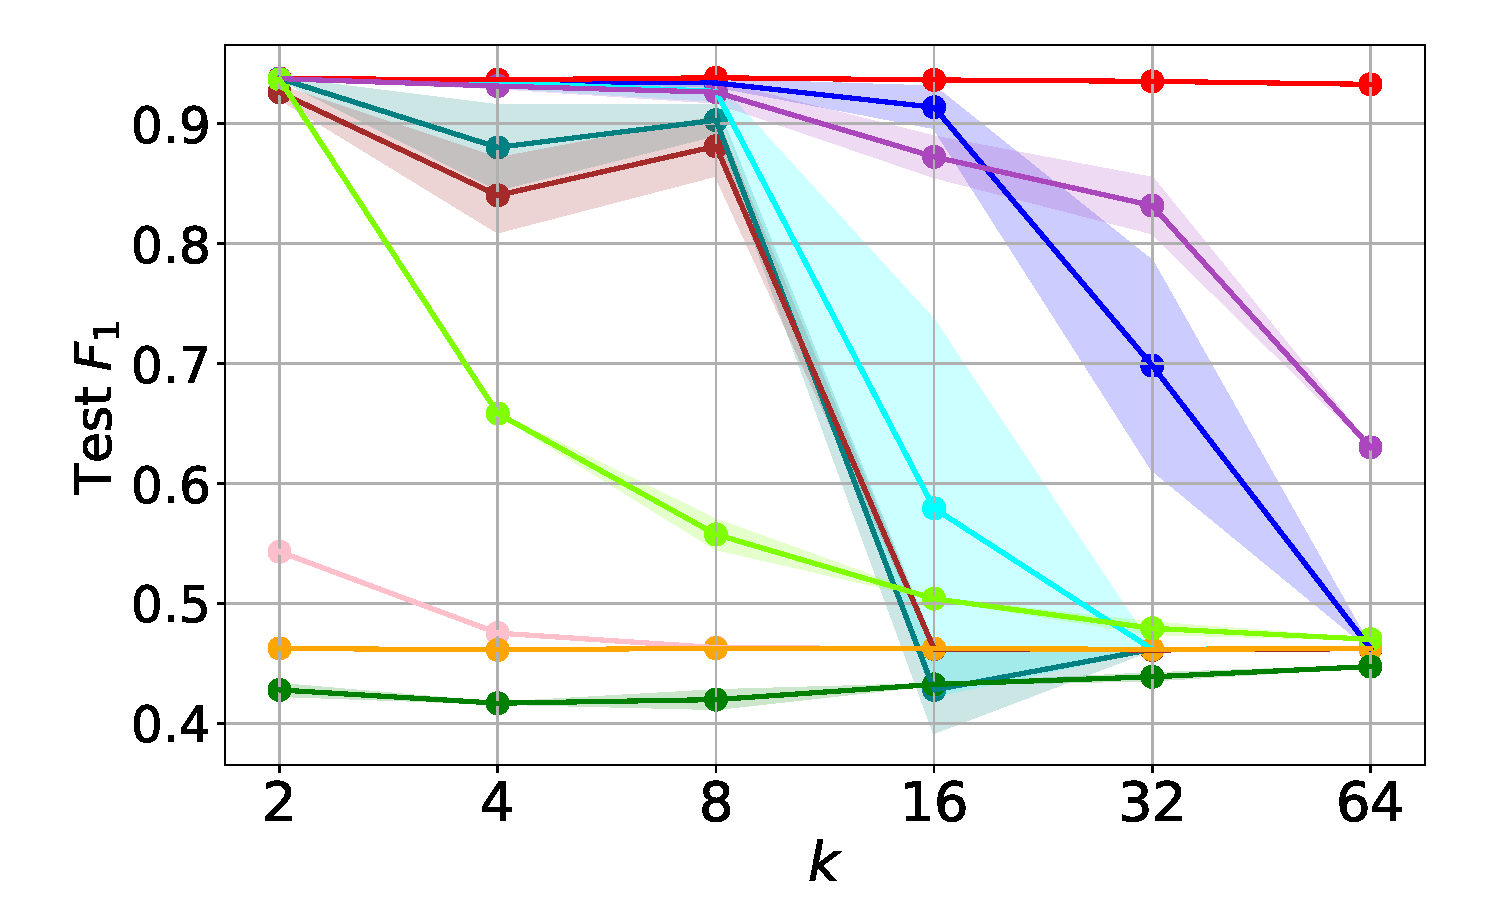
\includegraphics[width=0.35\linewidth]{figs/periodicity/sbm_sto/V2/(0.9, 0.01)(k, 1)All_test avg_f1.pdf}%
        \hspace{0.5cm}%
        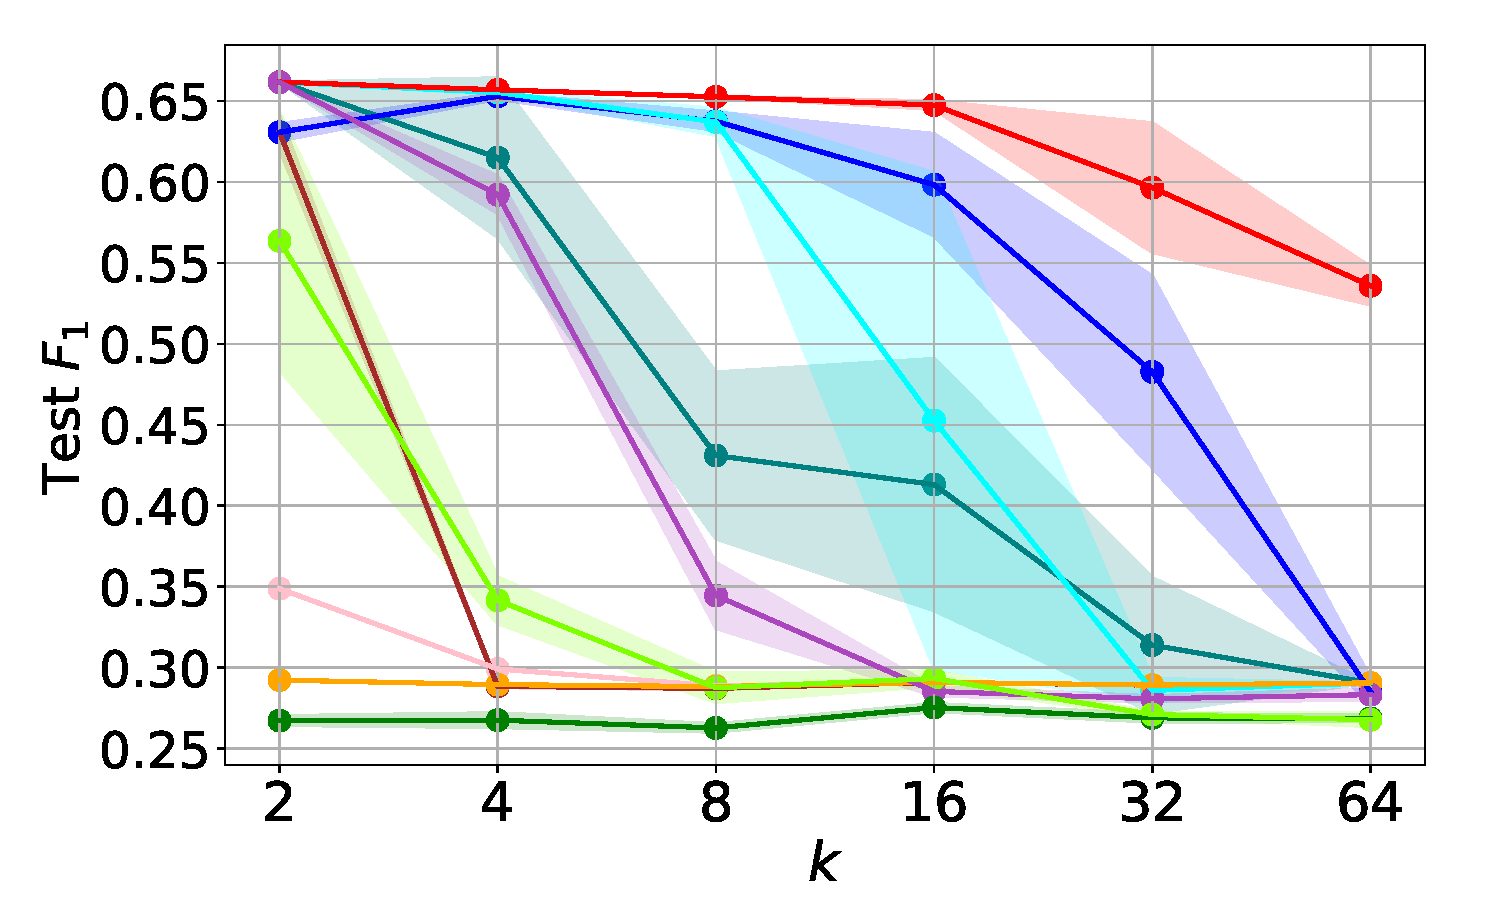
\includegraphics[width=0.35\linewidth]{figs/periodicity/sbm_sto/V2/(0.5, 0.01)(k, 1)All_test avg_f1.pdf}%
        %\hspace{1cm}%
        \raisebox{5mm}{
        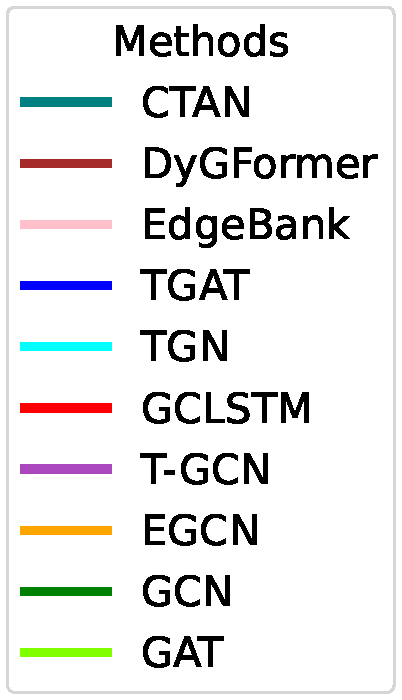
\includegraphics[width=0.08\linewidth]{figs/legends/CTDG DTDG all w edgebank wo persistence.pdf}}
    \caption{ Performance of TGL methods on the stochastic periodicity tasks~$\Psto{k,1}$ for different values of the intra-community edge probability: $p=0.9$ (left) and $p=0.5$ (right).
    % \mh{I don't understand why do we have p=0.5 here? what does it tell that the left plot is not telling us?
    % In text we say
    % "overall, the performance gap between models widens under lower intra-community density (p = 0.5)"
    % Which I don't think is true, at least it's not clearly visible in left and right plot
    % I suggest remove left hand plot or more it to appendix and remove the mentioned sentence.
    % }
    }
    \label{fig:(K,1)_overall_sto}
\end{figure}

